\documentclass{article}
\usepackage{enumitem}
\usepackage{graphicx}
%\graphicspath{{figs/}}
\usepackage{amsmath}
\usepackage{amsfonts}
\usepackage{float}
\usepackage{gensymb}
\let\vec\mathbf
\begin{document}
\title{Circles-10}
\begin{enumerate}
	\item A quadrilateral $ABCD$ is drawn to circumscribe a circle (see Figure-1). Prove that $AB + CD = AD + BC$.
ssssi	\begin{figure}[!htb]
		\centering
			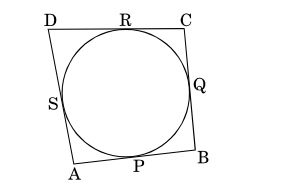
\includegraphics[width=\columnwidth]{figs/circ-1.png}
		
		\caption{}
		\label{fig:circ-1}
	\end{figure}
	\item Draw a pair of tangents to a circle of radius $4 cm$ which are inclined to each other at an angle of 45\degree.	
	\item A point $\vec{T}$ is $13 cm$ away from the centre of a circle. The length of the tangent drawn from $\vec{T}$ to the circle is $12 cm$. Find the radius of the circle.
	\item Two tangents $TP$ and $PQ$ are drawn to a circle with centre $\vec{O}$ from an external point $\vec{T}$. Prove that $\angle PTQ = 2 \angle OPQ$.
	\item $PQ$ is a tangent to a circle with centre $\vec{O}$ at the point $\vec{P}$ on the circle. If $\triangle OPQ$ is an isosceles triangle, then find $\angle OQP$.
	\item Two concentric circles have radii $10 cm$ and $6 cm$. Find the length of the chord of the larger circle which touches the smaller circle.
	\item If tangents $PA$ and $PB$ from an external point $\vec{P}$ to a circle with centre $\vec{O}$ are inclined to each other at an angle of 70\degree, then find $\angle POA$.
	\item $ABC$ is right triangle, right-angled at $\vec{B}$ with $BC = 6 cm$ and $AB = 8 cm$. A circle with centre $\vec{O}$ and radius $r$ cm has been inscribed in $\triangle ABC$ as shown in the figure. Find the value of $r$.
		\begin{figure}[H]
			\centering
			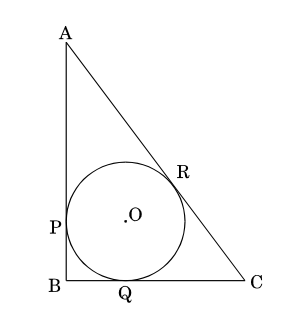
\includegraphics[width=\columnwidth]{figs/circ-2.png}
			\caption{}
			\label{fig:circ-2}
		\end{figure}
	\item Draw a circle of radius $5 cm$. From a point $8 cm$ away from its centre, construct a pair of tangents to the circle.
	\item In the given figure, $PT$ and $PS$ are tangents to a circle with centre $\vec{O}$, from a point $\vec{P}$, such that $PT = 4 cm$ and $\angle TPS = 60$\degree. Find the length of the chord $TS$. Also, find the radius of the circle.
		\begin{figure}[H]
			\centering
			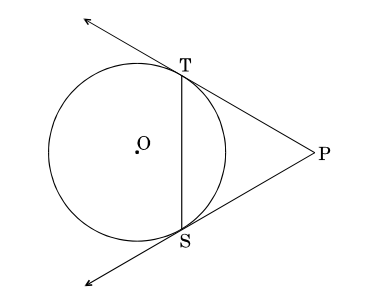
\includegraphics[width=\columnwidth]{figs/circ-3.png}
			\caption{}
			\label{fig:circ-3}
		\end{figure}
	\item \begin{enumerate}[label=(\alph*)]
			\item In a right triangle $ABC$, right-angled at $\vec{B}$, $BC = 6 cm$ and $AB = 8 cm$. A circle is inscribed in the $\triangle ABC$. Find the radius of the incircle.
			\item Two circles touch externally at $\vec{P}$ and $AB$ is a common tangent, touching one circle at $\vec{A}$ and the other at $\vec{B}$. Find the measure of $\angle APB$.
		\end{enumerate}
	\item From an external point $\vec{P}$, tangents $PQ$ and $PR$ are drawn to a circle with centre $\vec{O}$, touching the circle at $\vec{Q}$ and $\vec{R}$. If $\angle QOR = 140$\degree, find the measure of $\angle QPR$.
	\item A circle touches all the sides of a quadrilateral $ABCD$. Prove that $AB + CD = DA + BC$.
	\item Write the steps of construction of a circle of diameter $6 cm$ and drawing of a pair of tangents to the circle from a point $5 cm$ away from the centre.
\end{enumerate}
\end{document}
                                                                                
